\begin{tikzpicture}
  \node at (0,0) {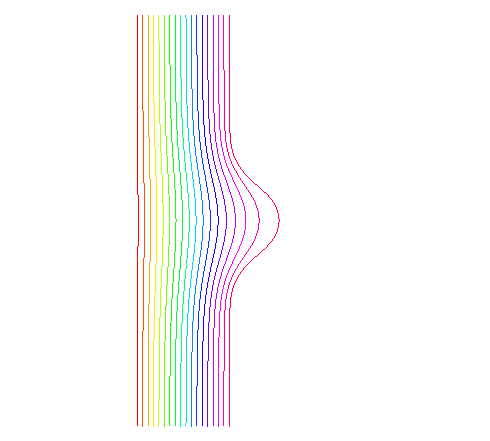
\includegraphics{gunfield.png}};
  \draw [fill=blue!40]
    (-1.4,-3.1)
    -- ++(0,6.2)
    -- ++(-1.1,0)
      node [above, pos=0.5] {$-V$}
    -- ++(0,-6.2)
      node [right=0.5, rotate=90, pos=0.7] {Photocathode}
    -- cycle
  ;
  \fill
    (-1.4,-0.4)
    -- ++(0,0.8)
      coordinate [pos=0.5] (source)
    -- ++(-0.1,0)
    -- ++(0,-0.8)
    -- cycle
  ;
  \draw [fill=blue!40, radius=0.7]
    (-0.15,-2.45)
    -- ++(0,1.35)
    arc [start angle=180, end angle=90]
    -- ++(0.4,0)
    -- ++(0,-2.75)
    -- ++(-0.4,0)
    arc [start angle=270, end angle=180]
    -- cycle
  ;
  \draw [fill=blue!40, radius=0.7]
    (-0.15,1.1)
    -- ++(0,1.35)
    arc [start angle=180, end angle=90]
    -- ++(0.4,0)
      node [pos=0.1,above] {$0V$}
    -- ++(0,-2.75)
    -- ++(-0.4,0)
    arc [start angle=270, end angle=180]
    -- cycle
  ;
  \draw [green, <-, ultra thick]
    (source)
    -- ++(-70:4)
      node [black,right] {Laser}
  ;
\end{tikzpicture}
